\documentclass{article}
\usepackage[utf8]{inputenc}
\usepackage{graphicx}
\usepackage[section]{placeins}
\usepackage{booktabs}


\title{Traffic stops at Rhode Island}
\author{Laura Barranco Navarro }
\date{February 2022}

\begin{document}

\maketitle
\newpage
\tableofcontents
\newpage
\section{Reason for speed by gender}

 \begin{figure}
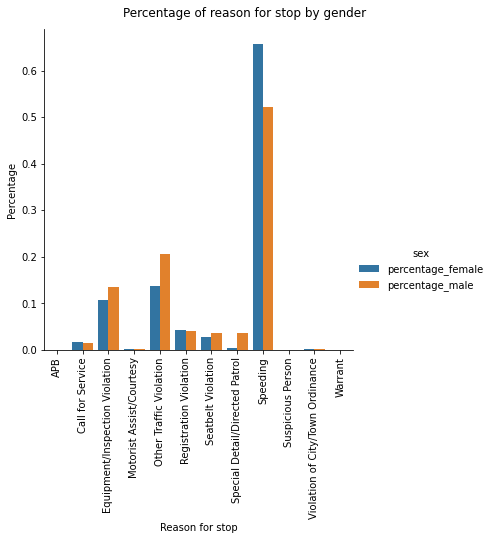
\includegraphics[width=0.8\textwidth]{../figures/reason_gender.png}
\end{figure}   



\begin{tabular}{lrr}
\toprule
                  Reason for stop & Female & Male \\
\midrule
                        Speeding &  0.657 & 0.522 \\
         Other Traffic Violation &  0.137 & 0.207 \\
  Equipment/Inspection Violation &  0.107 & 0.135 \\
          Registration Violation &  0.043 & 0.041 \\
              Seatbelt Violation &  0.027 & 0.037 \\
                Call for Service &  0.018 & 0.015 \\
  Special Detail/Directed Patrol &  0.005 & 0.037 \\
        Motorist Assist/Courtesy &  0.003 & 0.002 \\
Violation of City/Town Ordinance &  0.002 & 0.002 \\
                             APB &  0.001 & 0.001 \\
               Suspicious Person &  0.001 & 0.001 \\
                         Warrant &  0.000 & 0.000 \\
\bottomrule
\end{tabular}
\FloatBarrier

\section{Outcome of speeding by gender}
 \begin{figure}
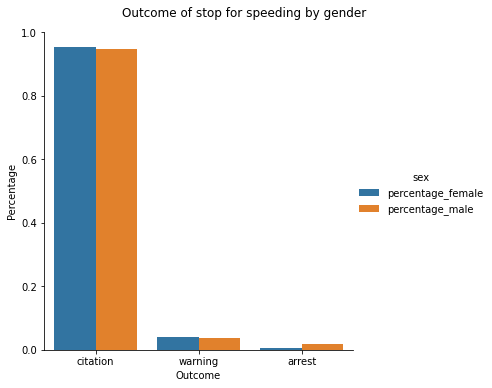
\includegraphics[width=0.8\textwidth]{../figures/speeding_outcome_gender.png}
\end{figure}

\begin{tabular}{lrr}
\toprule
 Outcome & Female &  Male \\
\midrule
citation &  0.955 & 0.947 \\
 warning &  0.039 & 0.036 \\
  arrest &  0.006 & 0.017 \\
\bottomrule
\end{tabular}

\FloatBarrier
\end{document}
